\documentclass{beamer}
\usepackage{relsize}
\usepackage{color}
\usepackage{rotating}

\usepackage{listings}
\usetheme{CambridgeUS}
%\usepackage{beamerthemesplit} % new 
\usepackage{enumitem}
\usepackage{amsmath}                    % See geometry.pdf to learn the layout options.\includeonlyframes{current}
\usepackage{amsthm}                   % See geometry.pdf to learn the layout options. There 
\usepackage{amssymb}                    % See geometry.pdf to learn the layout options. 
\usepackage[utf8]{inputenc} 
\usepackage{graphicx}
\usepackage[english,bulgarian]{babel}
\usepackage{changepage} 

\lstset{language=C++,
                basicstyle=\ttfamily,
                keywordstyle=\color{blue}\ttfamily,
                stringstyle=\color{red}\ttfamily,
                commentstyle=\color{green}\ttfamily,
                morecomment=[l][\color{magenta}]{\#}
}

\setbeamertemplate{itemize items}[circle]

\newtheorem{mydef}{Дефиниция}[section]
\newtheorem{lem}{Лема}[section]
\newtheorem{thm}{Твърдение}[section]
\newtheorem*{remark}{}

\DeclareMathOperator{\restrict}{\upharpoonright}

\setitemize{label=\usebeamerfont*{itemize item}%
  \usebeamercolor[fg]{itemize item}
  \usebeamertemplate{itemize item}}

\setbeamercovered{transparent}



\begin{document}
\title[Увод в програмирането]{Работа с текстови файлове} 
\author{Калин Георгиев}
\frame{\titlepage} 


\section{Файлове}


\begin{frame}
\centerline{Файлове}
\end{frame}


\begin{frame}[fragile]
\frametitle{``Физически'' файлове}


\begin{center}
   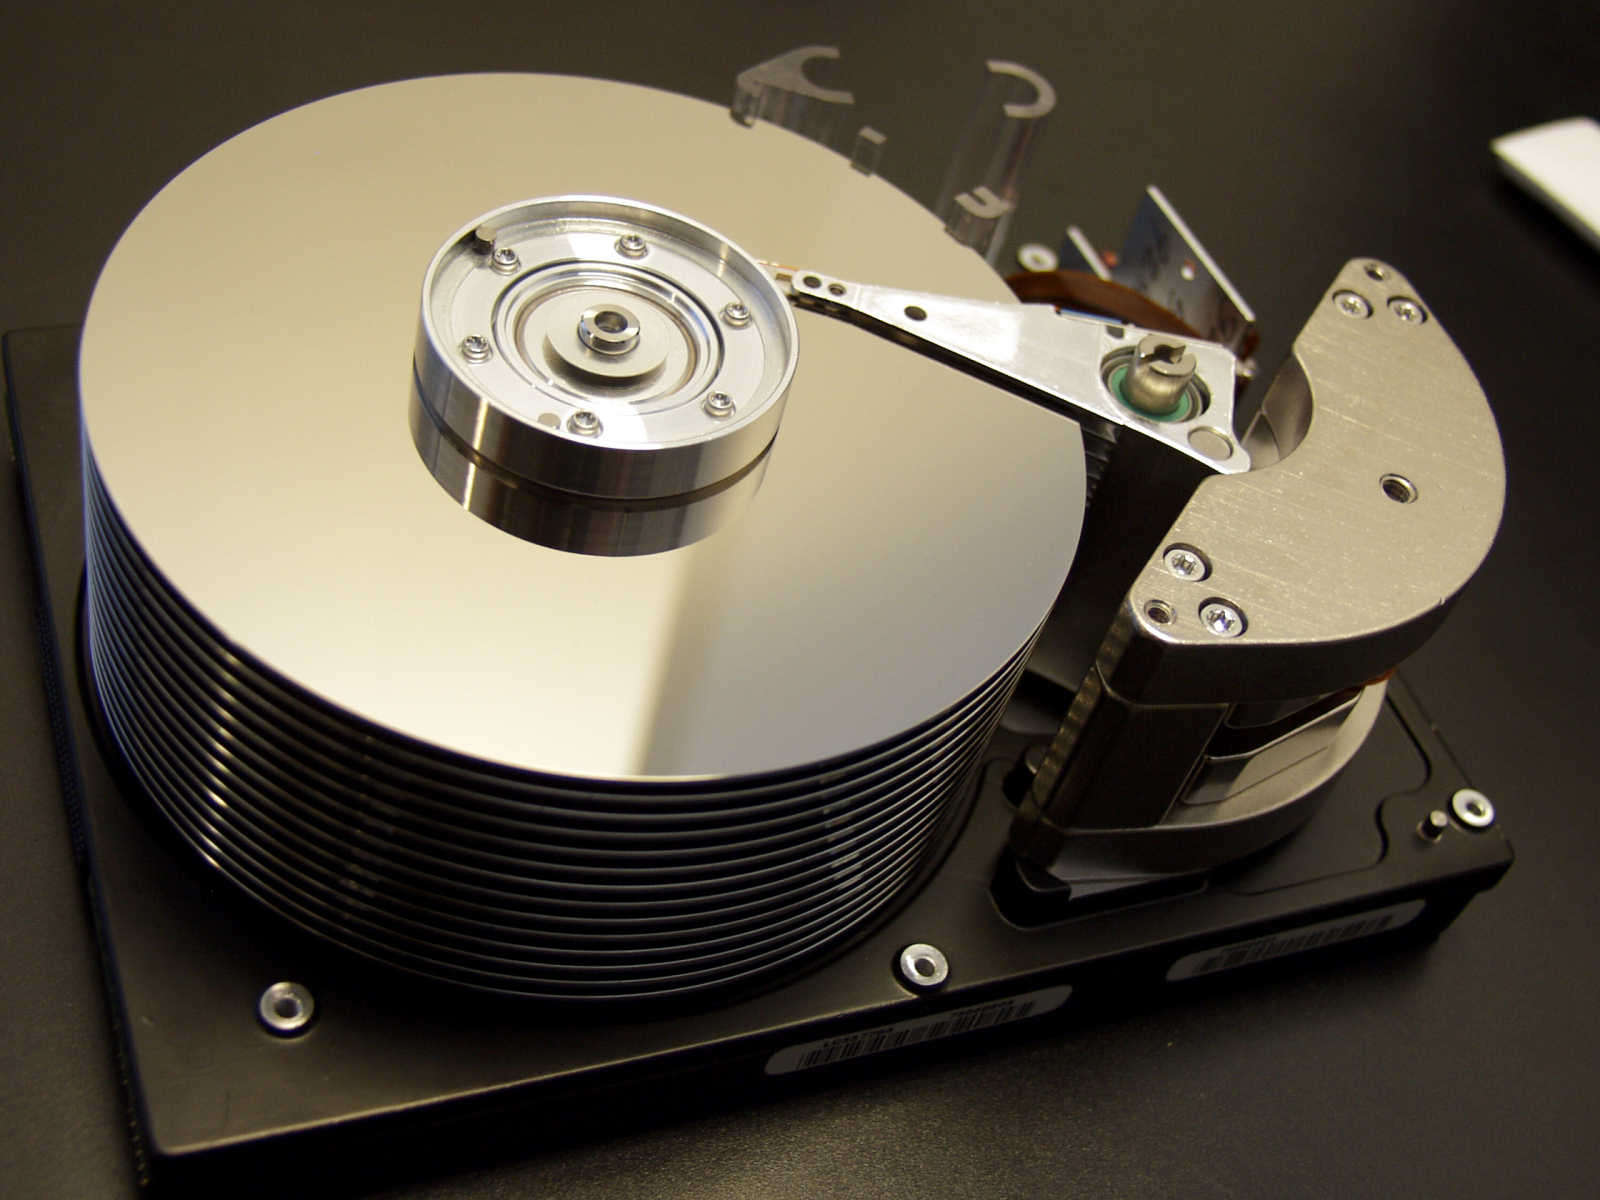
\includegraphics[width=7cm]{images/harddisk}
\end{center}

\end{frame}

\begin{frame}[fragile]
\frametitle{``Физически'' файлове}


\begin{center}
   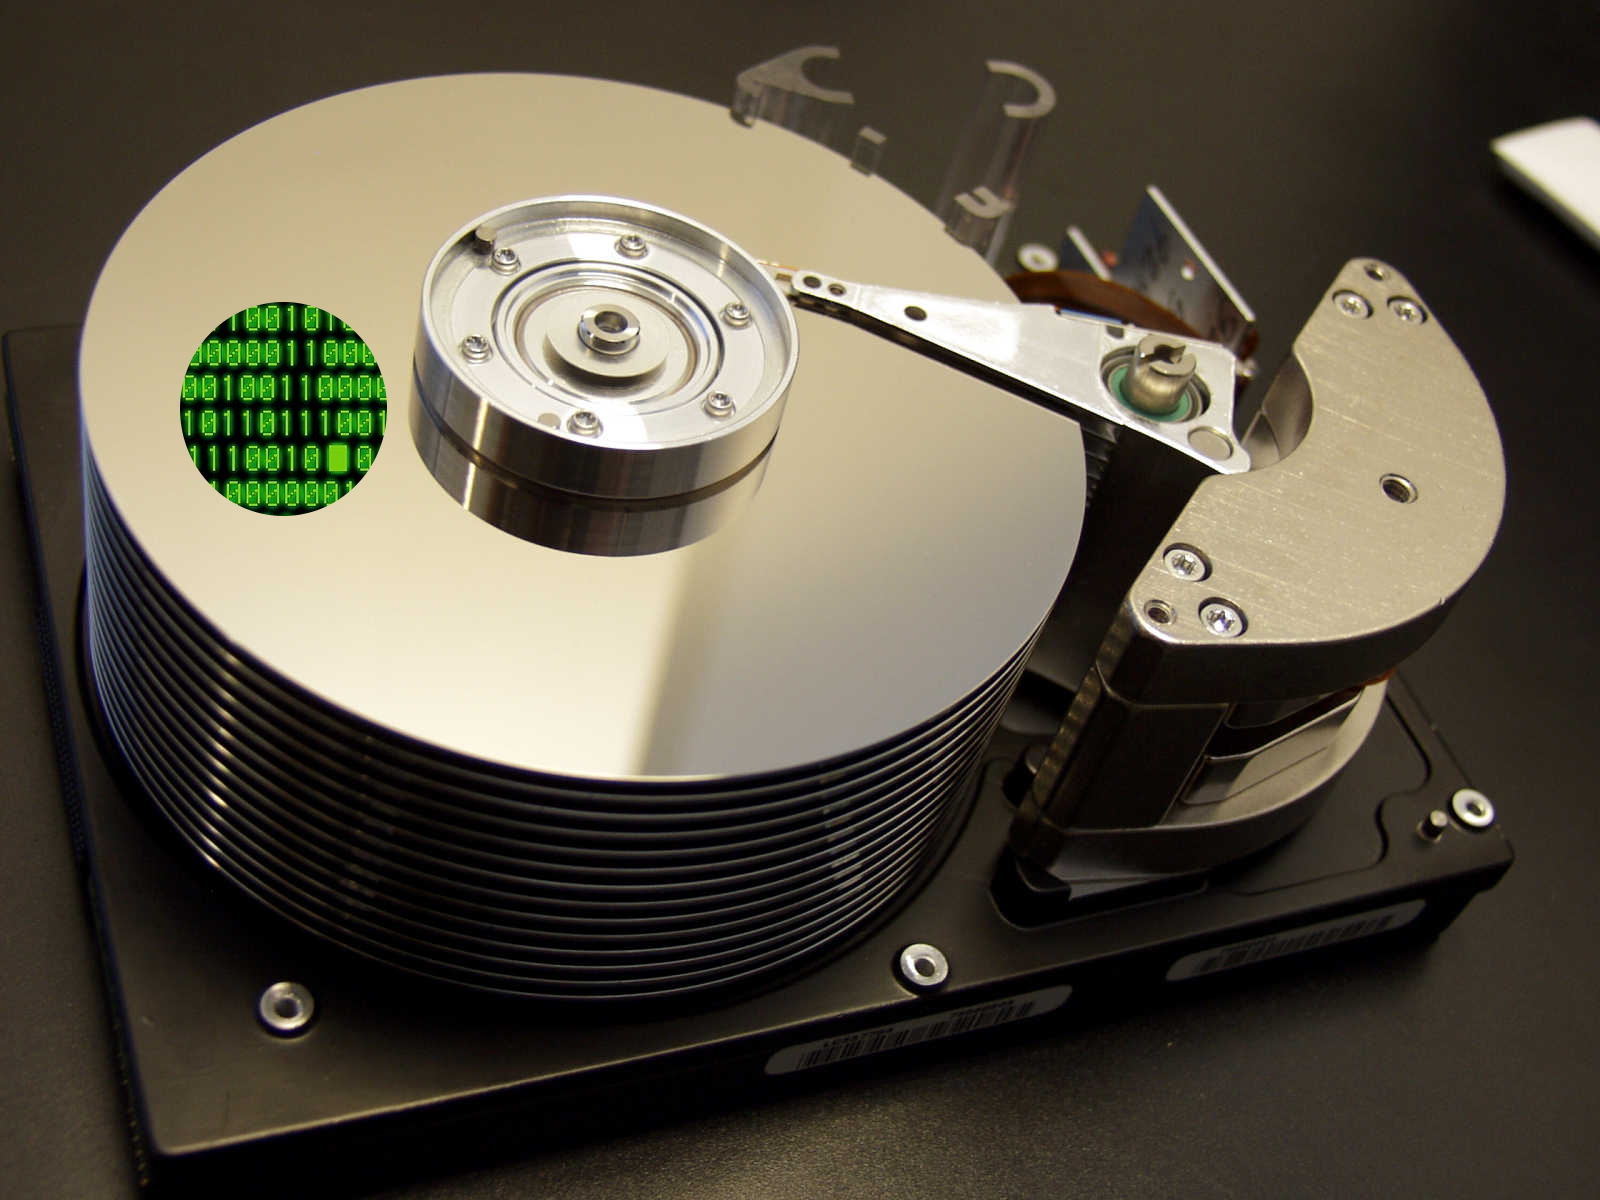
\includegraphics[width=7cm]{images/harddisk-oneszeros}
\end{center}

\end{frame}


\begin{frame}[fragile]
\frametitle{``Логически'' файлове}


\begin{center}
   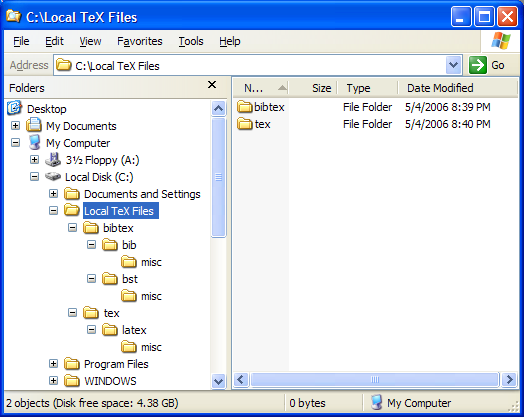
\includegraphics[width=7cm]{images/directorytree}
\end{center}

\end{frame}


\begin{frame}[fragile]
\frametitle{Данни във файл vs. данни в паметта}


\begin{columns}[t]
  \begin{column}{0.5\textwidth}
\begin{center}

\begin{flushleft}
\relscale{0.65}
\begin{itemize}
  \item персистентни
  \item бавни
  \item големи обеми 
\end{itemize}
\end{flushleft}

\vspace{20px}

   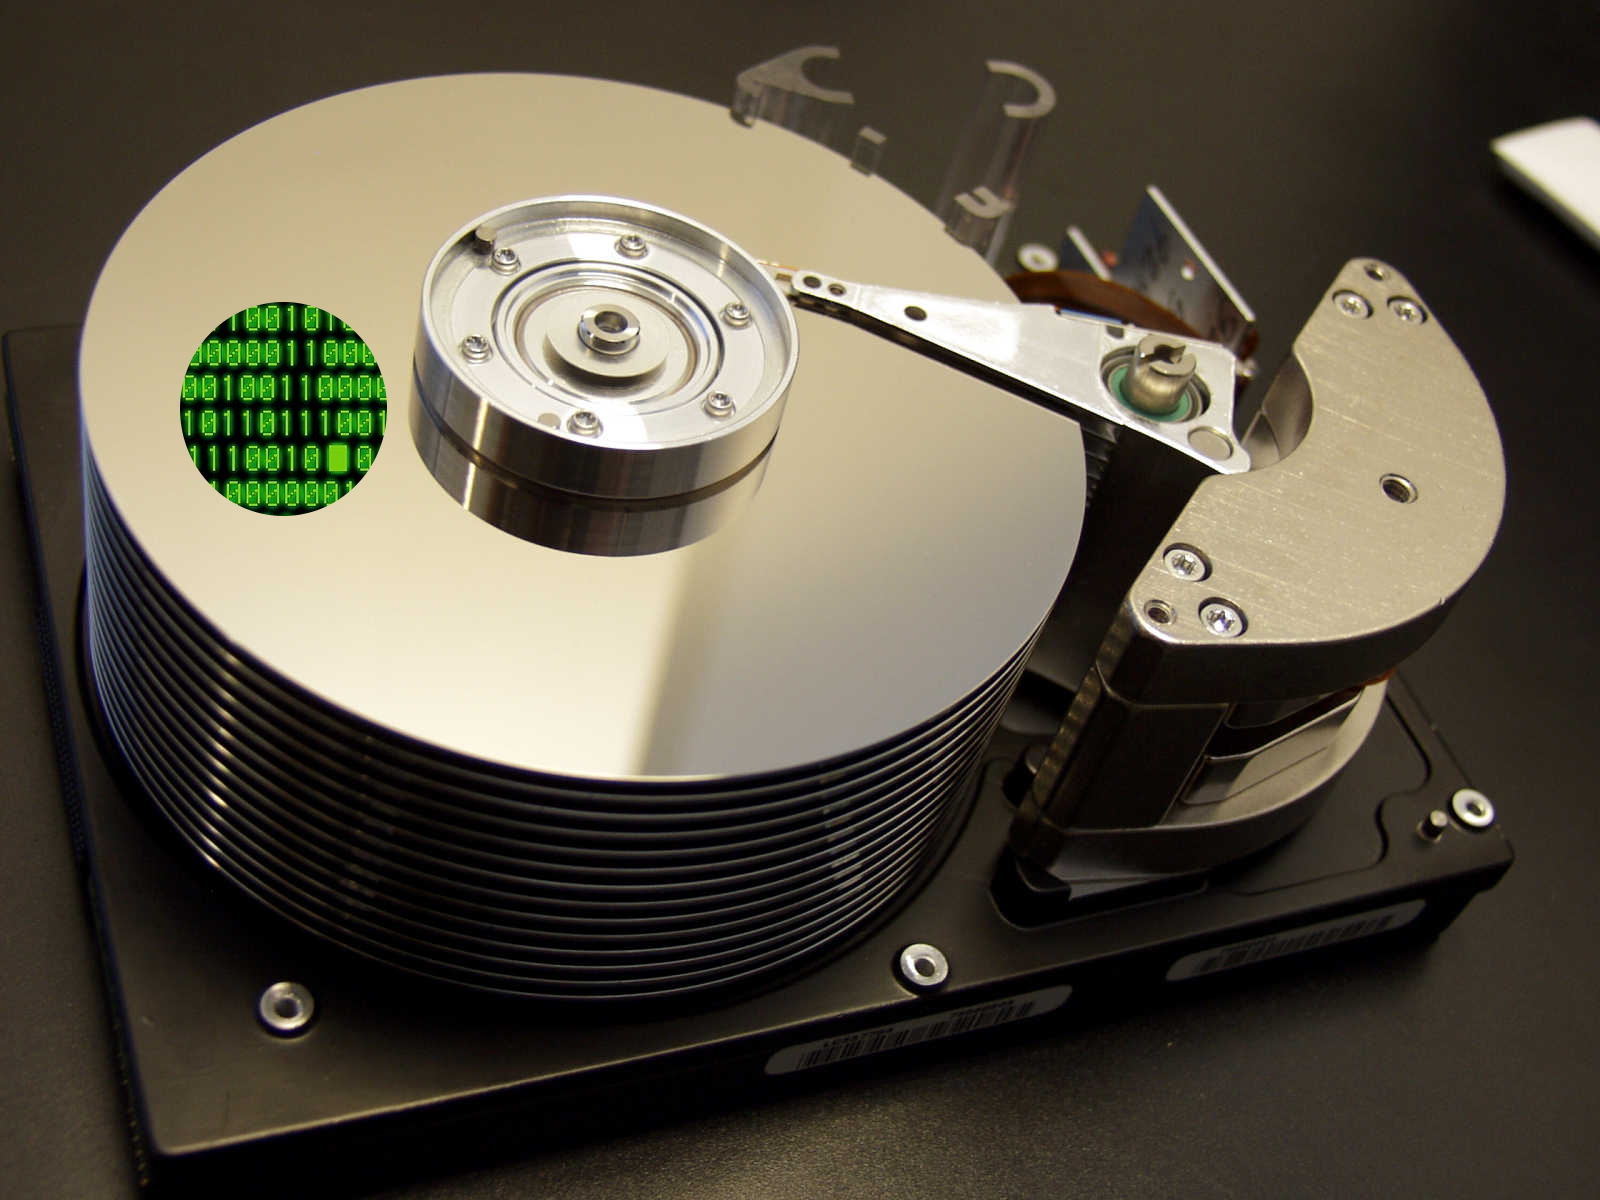
\includegraphics[width=5cm]{images/harddisk-oneszeros}
\end{center}
  \end{column}
  \begin{column}{0.5\textwidth}
\begin{center}

\begin{flushleft}
\relscale{0.65}
\begin{itemize}
  \item до приключване на програмата
  \item бързи
  \item по-ограничени обеми  
\end{itemize}
\end{flushleft}
\vspace{20px}


   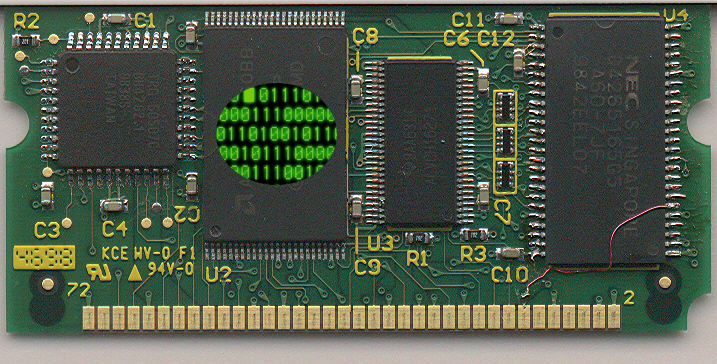
\includegraphics[width=5cm]{images/ramchip-oneszeros}
   \pause
\begin{flushleft}
\relscale{0.65}
\begin{lstlisting}
int i;
int intarr[100];
Student student;
Student studentarr[100];
\end{lstlisting}
\end{flushleft}   
\end{center}
  \end{column}
\end{columns}




\end{frame}


\begin{frame}
\centerline{Работа с файлове: трансфер на данни между}
\centerline{оперативната памет и постоянната памет}
\begin{columns}[t]
  \begin{column}{0.5\textwidth}
\begin{center}

   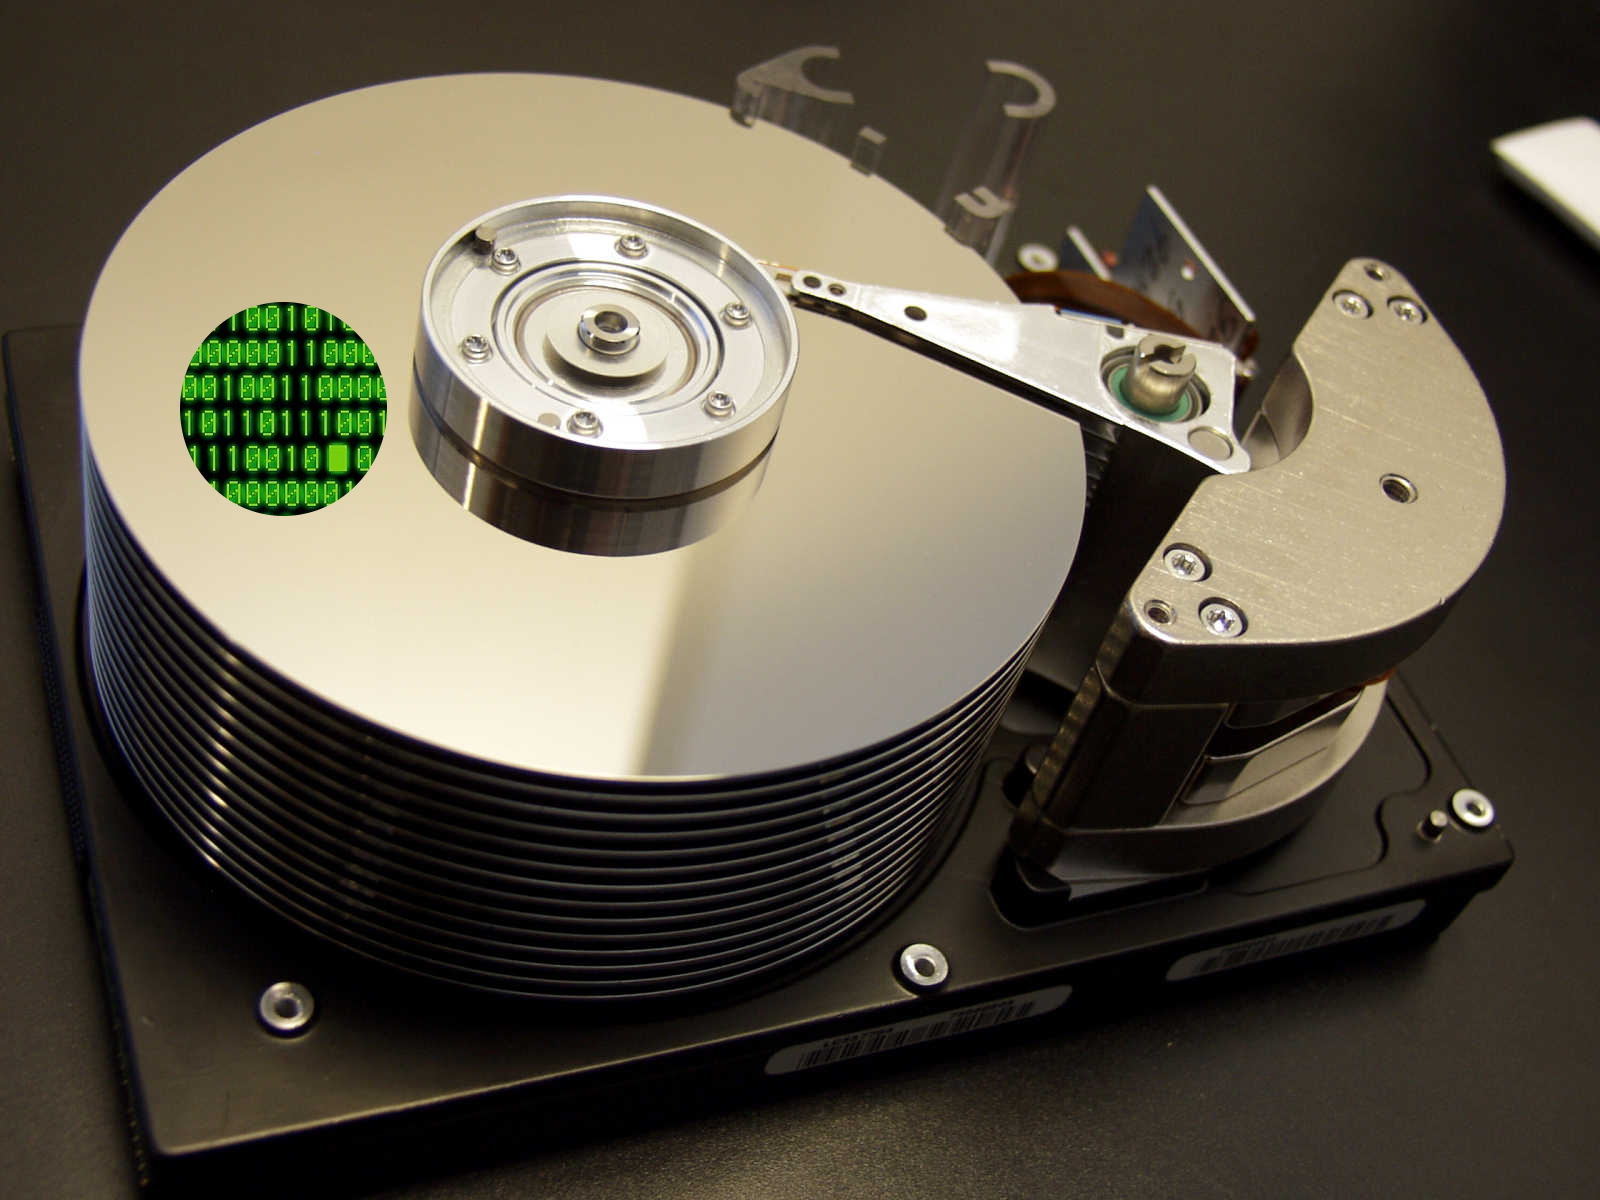
\includegraphics[width=3cm]{images/harddisk-oneszeros}
\end{center}
  \end{column}
  \begin{column}{0.5\textwidth}
\begin{center}

   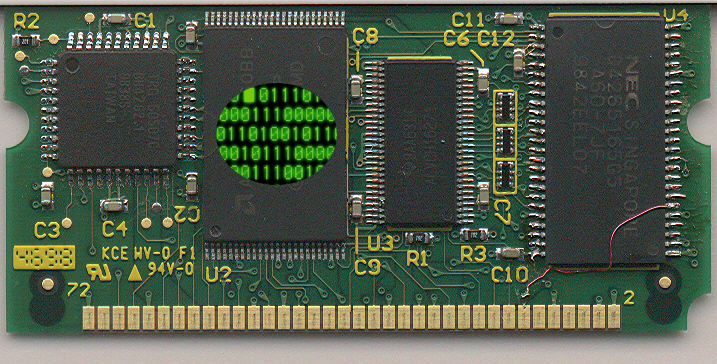
\includegraphics[width=3cm]{images/ramchip-oneszeros}
\end{center}
  \end{column}
\end{columns}

\end{frame}

\section{Текстови файлове}

\begin{frame}
\centerline{Текстови файлове}
\end{frame}


\begin{frame}[fragile]
\frametitle{struct Student}



\begin{columns}[t]
  \begin{column}{0.5\textwidth}
      \vspace{-350px}
      \begin{flushleft}
      \relscale{0.85}
      \begin{lstlisting}
      struct Student
      {
        int fn;
        char name[100];
        double grade;
        //others
      };
      \end{lstlisting}
      \end{flushleft} 
  \end{column}
  \begin{column}{0.5\textwidth}
  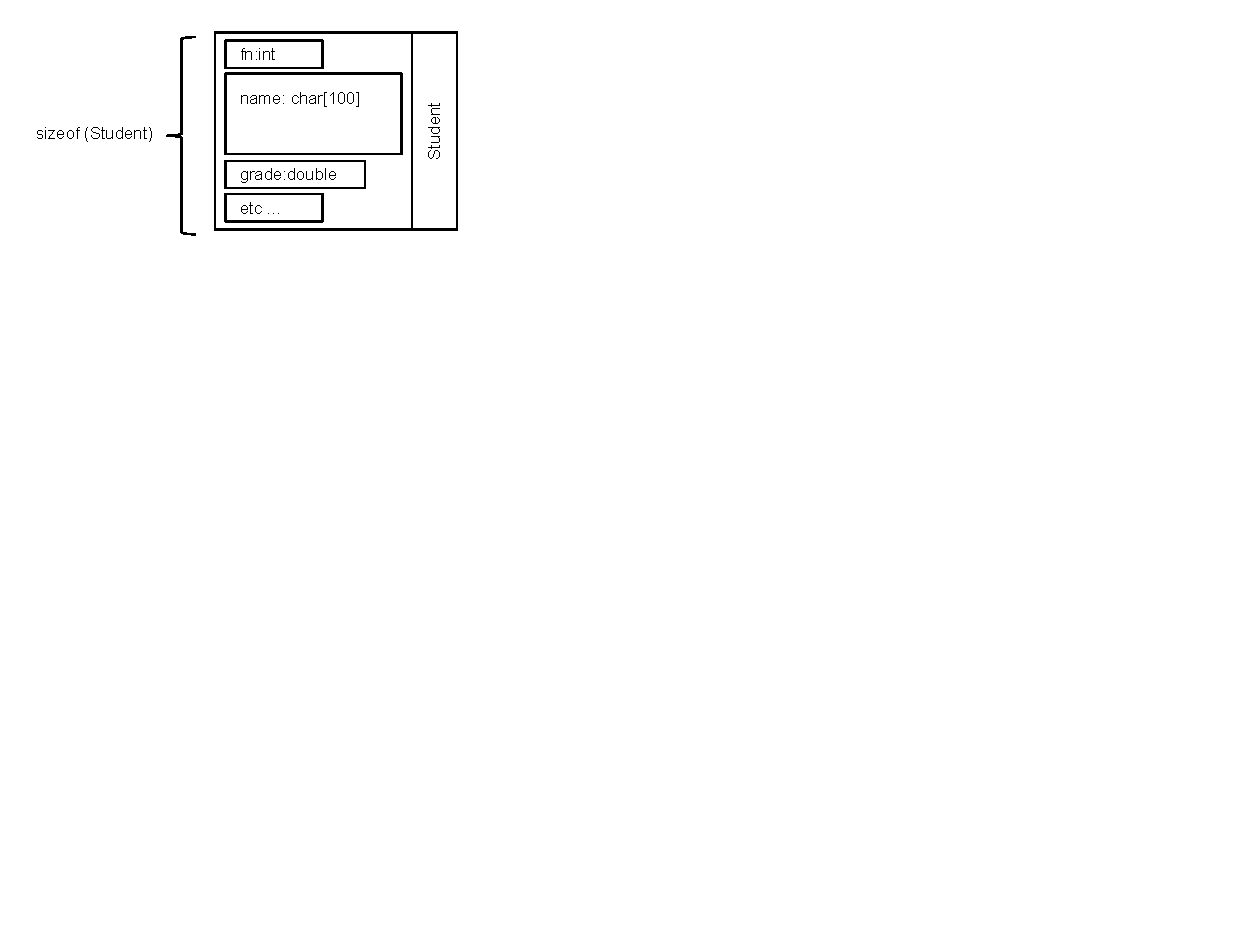
\includegraphics[width=16cm]{images/structstudent}
  \end{column}
\end{columns}


\end{frame}


\begin{frame}[fragile,label=current]
\frametitle{Изход на конзолата}



\begin{columns}[t]
  \begin{column}{0.5\textwidth}
      \vspace{-150px}
      \begin{flushleft}
      \relscale{0.65}
      \begin{lstlisting}
Student students[100];
//...
for (int i = 0; i < 3; i++)
{
    cout << students[i].fn 
         << " "
         << students[i].name 
         << endl 
         << students[i].grade 
         << endl;
}
      \end{lstlisting}
      \end{flushleft} 
  \end{column}
  \begin{column}{0.5\textwidth}
  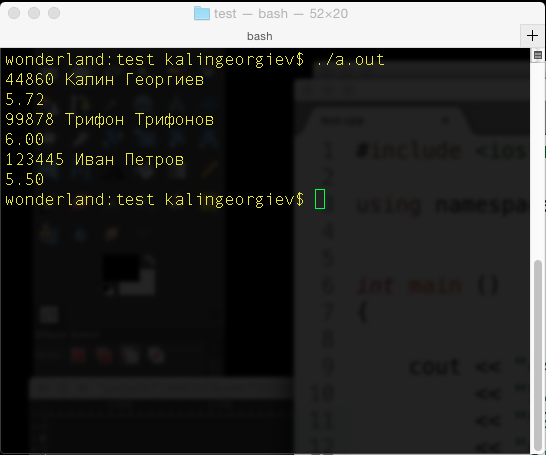
\includegraphics[width=5cm]{images/consoleout}
  \end{column}
\end{columns}


\end{frame}



\begin{frame}[fragile]
\frametitle{Изход в текстов файл}



\begin{columns}[t]
  \begin{column}{0.5\textwidth}
      \vspace{-150px}
      \begin{flushleft}
      \relscale{0.65}
      \begin{lstlisting}
Student students[100];
//...
ofstream out_file ("myfile.txt");
for (int i = 0; i < 3; i++)
{
  out_file << students[i].fn 
           << " "
           << students[i].name 
           << endl 
           << students[i].grade 
           << endl;
}
      \end{lstlisting}
      \end{flushleft} 
  \end{column}
  \begin{column}{0.5\textwidth}
  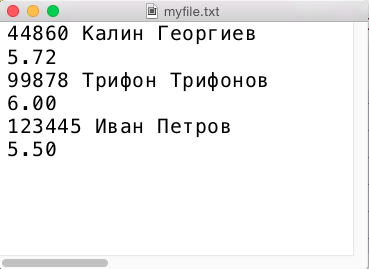
\includegraphics[width=5cm]{images/textedit}
  \end{column}
\end{columns}


\end{frame}




\begin{frame}[fragile]
\frametitle{Вход от конзолата}



\begin{columns}[t]
  \begin{column}{0.5\textwidth}
      %\vspace{-150px}
      \begin{flushleft}
      \relscale{0.65}
      \begin{lstlisting}
Student students[100];
//...
for (int i = 0; i < 3; i++)
{
    cin >> students[i].fn;
    cin.getline (students[i].name,100);
    cin >> students[i].grade;
}
      \end{lstlisting}
      \end{flushleft} 
  \end{column}
  \begin{column}{0.5\textwidth}
  \relscale{0.6}
\begin{verbatim}
44860 Калин Георгиев
5.72 99878 Трифон Трифонов
6.00 123445 Иван Петров
5.50

\end{verbatim}
  \end{column}
\end{columns}


\end{frame}





\begin{frame}[fragile]
\frametitle{Вход от текстов файл}



\begin{columns}[t]
  \begin{column}{0.6\textwidth}
      %\vspace{-150px}
      \begin{flushleft}
      \relscale{0.65}
      \begin{lstlisting}
Student students[100];
//...
ifstream in_file ("myfile.txt");
for (int i = 0; i < 3; i++)
{
  in_file >> students[i].fn;
  in_file.getline (students[i].name,100);
  in_file >> students[i].grade;
}
      \end{lstlisting}
      \end{flushleft} 
  \end{column}
  \begin{column}{0.4\textwidth}

  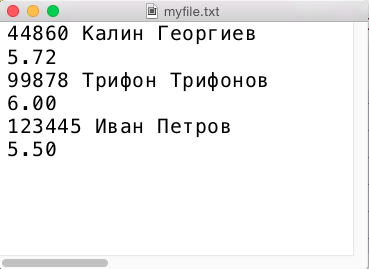
\includegraphics[width=4.5cm]{images/textedit}
  \end{column}
\end{columns}
\end{frame}




\begin{frame}[fragile]
\frametitle{Вход/изход от текстов файл}



\begin{columns}[t]
  \begin{column}{0.6\textwidth}
      %\vspace{-150px}
      \begin{flushleft}
      \relscale{0.65}
      \begin{itemize}
        \item последователно четене и писане
        \item достъп до елемент по индекс?
        \item изтриване на елемент?
      \end{itemize}
      \end{flushleft} 
  \end{column}
  \begin{column}{0.4\textwidth}

  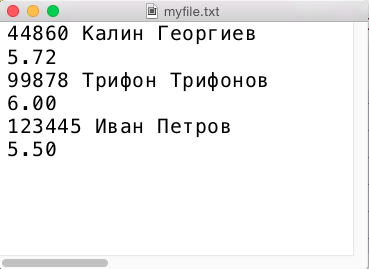
\includegraphics[width=4.5cm]{images/textedit}
  \end{column}
\end{columns}
\end{frame}


\begin{frame}
\centerline{Благодаря за вниманието!}
\end{frame}

\end{document}




\begin{columns}[t]
  \begin{column}{0.2\textwidth}

  \end{column}
  \begin{column}{0.8\textwidth}

  \end{column}
\end{columns}
